\chapter{Statistical Analysis} \label{chapter:statistical-analysis}
Having prepared the bond data and matched it with the stocks, some statistical analysis can now be performed. In particular, we are interested in summary statistics of corporate bond returns, as well as in the analysis of the lead-lag relationship of corporate bond and stock returns. For this, the returns themselves need to be calculated from daily prices first. Additionally, as the matching has so far only been done for static data, it needs to be extended to historical return data as well. All in all, the following procedure for the statistical analysis arises: 
\begin{enumerate}
	\item Calculate monthly bond returns
	\item Match bond and equity returns
	\item Calculate summary statistics
	\item Analyse lead-lag relationship
\end{enumerate}

\section{Monthly Bond Returns}
In order to calculate the monthly bond returns, the following formula will be used: \\
$R_{n} = \dfrac{P_{n}}{P_{n-1}}$, \\ where $R_{n}$ stands for bond return for month $n$, and $P_{n}$ for the bond price on last day of month $n$. 
To implement the formula in Stata, in the time series bond data only the last price of each bond for each month needs to be kept. The rest of the data can be dropped, as it is not relevant for the current analysis. The pricing parameter which will be used to calculate the returns is \textit{MPD}. It represents the Datastream Selected Default Price, and is the most reliable price parameter in the extracted database. Other price parameters, such as e.g. \textit{CP} (Clean Price), have significantly more missing values and are thus less suited for the purpose. Having kept the last monthly prices, a variable group consisting of the variables \textit{dscd} and \textit{month} has to be generated (\textit{egen} \textit{group} command). This group can then be set as a Stata time-series (\textit{tsset}). Based on the time-series, the monthly return variable can be generated with the introduced formula. The Stata do file for the task can be found in. %TODO  ref do_generate_monthly_returns

\section{Matching Bond and Equity Returns}
To match the bond and equity returns with each other, we can make use of the matching that we accomplished in chapter \ref{chapter:matching}. For this, we load the corporate bond returns, which we just calculated, into Stata. These bond returns can then be merged with the existing matching over the $bond_dscd$ parameter, as shown in Fig. \ref{fig:matching-returns}. 
\begin{figure}[h]
	\centering
	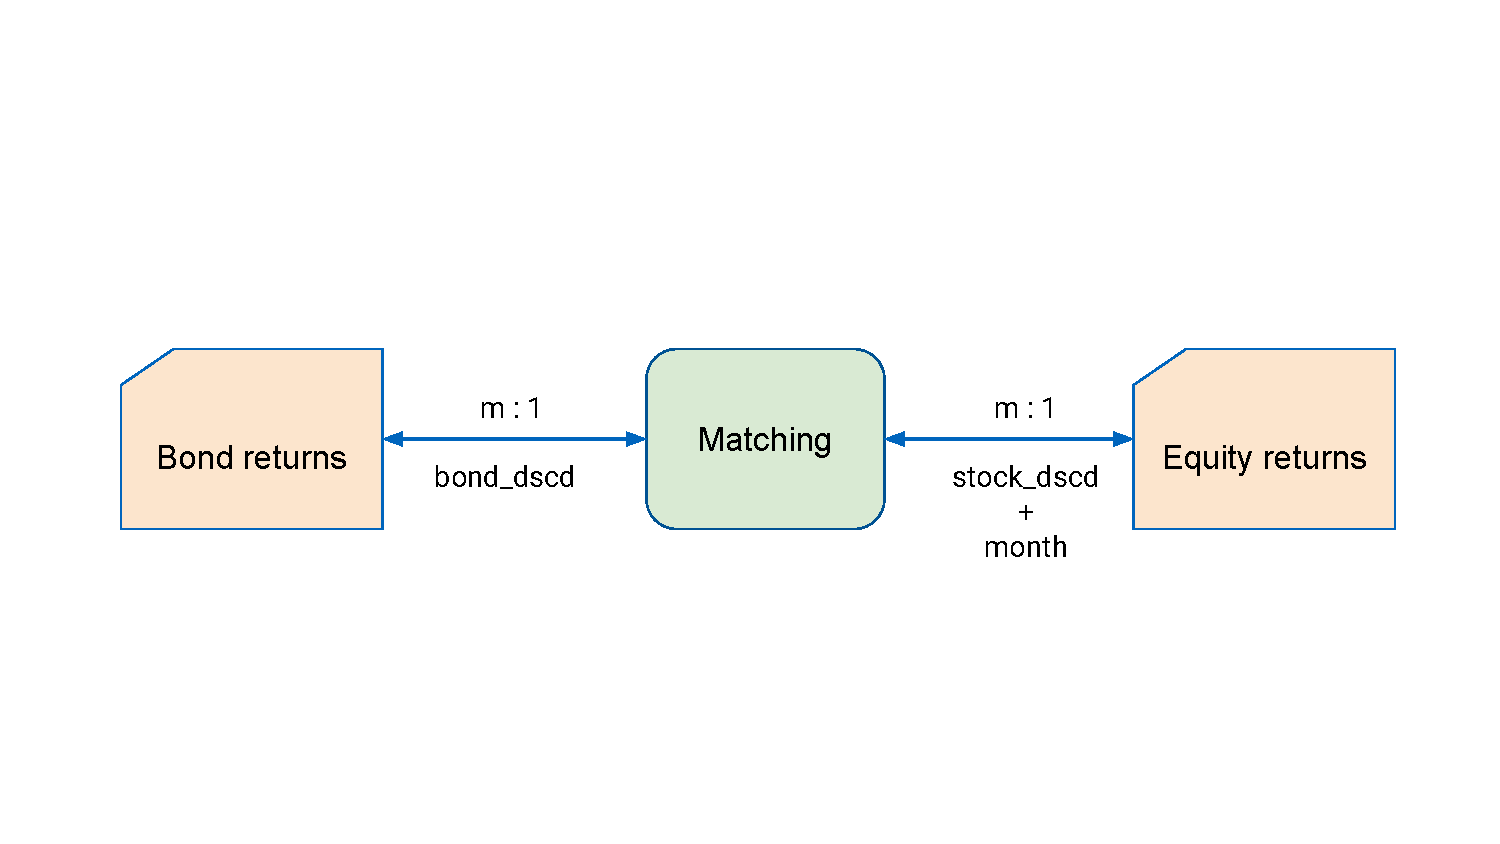
\includegraphics[trim={0 4.5cm 0 5cm},clip,width=1.0\linewidth]{figures/matching-returns.pdf}
	\caption{Matching of Bond and Equity Returns}
	\label{fig:matching-returns}
\end{figure}
After that, the resulting dataset has to be merged with the provided stock time series data, which also includes the required monthly stock returns. This merge should take place over the two parameters $stock_dscd$ and $month$. This is because we want the bond and stock returns to be comparable for one and the same month later on. When executing the merges in Stata, keep in mind to make sure that the Datastream code parameter is named the same in the bond dataset and the matching (i.e. $bond_dscd$), and similarly for the stocks and the matching (i.e. $stock_dscd$). Otherwise, the matching will fail. The bonds-matching merge is performed on a M-to-1 relation, because multiple bonds can be mapped to the same equity over the issuing company. The merge with the equities is performed on a M-to-1 relation as well for the same reason. The resulting database builds the foundation for further statistical analysis. 

\section{Summary Statistics} \label{section:summary-statistics}



\section{Lead-Lag Relationship} \label{section:lead-lag-relationship}











